\documentclass{article}
\usepackage[utf8]{inputenc}

\title{\textbf{Engineering Visualization Software}
\linebreak Modeling and Analysis}
\author{Animesh Singh}
\date{January 2018}

\usepackage{natbib}
\usepackage{graphicx}
\usepackage{amsmath}
\usepackage{esvect}

\begin{document}

\maketitle 

\begin{abstract}
    This project aims at creating 2D projections of a given 3D model taken as an input and finding projections onto any defined cutting plane. The software package will also be able to recover the 3D model completely from the defined 2D projections provided to it as an input in a suitable format. This report will create a mathematical model to implement the same and will define the mathematical tools needed to carry this out. We make the assumption that if given the 2D representations, we will be given the point correspondence along with clear demarcation of edges. 
\end{abstract}
\section{Representation}
The \textbf{3D representation} of an object consisting of only straight lines can be made in terms a graph $G (V,E)$, such that all the vertices on the object are present on the graph and a cut/line between two vertices can be represented by an edge in the graph. The same object, on projection onto a plane, can be represented by a graph with vertices in 2 dimensions. In order to represent curved surfaces, the surface can be discretized into a number of points, each connected by short lines, which will give an approximation of a curve. Instead of the graph representation, we also considered having a matrix of all pixels needed to represent the entire surface and projecting this matrix. While this may be easier to give for a graphical interface, it would lead to unnecessary space usage and processing.\par
2 views of an object are \emph{necessary and sufficient} in order to completely describe a 3-D model given the 2 projections of the object, if every point has been labeled appropriately. Without loss of generality, we can assume that a given point P in 3-D has coordinates $(x,y)$ in one projection and $(y,z)$ in another. This allows us to uniquely determine the coordinates of the point as $(x,y,z)$. A line can also be uniquely determined by finding out the two end points of the line segment. 

\section{Orthographic views of a 3-D object}
This section focuses on finding the orthographic views of an object given its 3-D representation. The object may be oriented in any way with respect to the \emph{original coordinate system} and thus the coordinate system must be rotated to be in direction of the viewing plane and also must be translated in an appropriate way to change the position of the origin. Throughout this section, we will consider an arbitrary point $p$ represented as 
\[p = \begin{bmatrix}
x\\
y\\
z\\
1\\
\end{bmatrix}\]

\subsection{Translation}
Let us first consider the translation of coordinate axes from the origin to an arbitrary point $p'$. Thus the new coordinates of the points will be \[p - p' = \begin{bmatrix}
x-x'\\
y-y'\\
z-z'\\
1\\
\end{bmatrix}\]
Thus, we can use a translation matrix, $T(p')$ which can used to translate the coordinate axes to $p'$ through multiplication. 
\[T(p') = \begin{bmatrix}
1&0&0&-x'\\
0&1&0&-y'\\
0&0&1&-z'\\
0&0&0&1\\
\end{bmatrix}\]
\begin{center}
    $p-p' = T(p')*p$
\end{center}
\subsection{Rotation}
Let us first consider the rotation about the z-axis, of points in the x-y plane. Consider the point (x,y) 
\[x = r\cos{\theta} \,\,\,\,\, y = r\sin{\theta}\]
On rotation by angle $\phi$,
\[x' = r\cos{(\theta + \phi)} \,\,\,\,\, y' = r\sin{(\theta + \phi)}\]
Expanding and expressing it in matrix form,
\[\begin{bmatrix}
x'\\y'\\\end{bmatrix} = \begin{bmatrix}\cos{\theta}&-\sin{\theta}\\\sin{\theta}&\cos{\theta}\\\end{bmatrix}\begin{bmatrix}x\\y\\\end{bmatrix}\]
In order to orient the viewing direction normal to one of the planes, a rotation of the coordinate axes is required. A rotation by angle $\theta$ about the z-axis is accomplished by
\[R_z(\theta) = \begin{bmatrix}
\cos{\theta}&-\sin{\theta}&0&0\\
\sin{\theta}&\cos{\theta}&0&0\\
0&0&1&0\\
0&0&0&1\\
\end{bmatrix}\]
Similarly, 
\[R_x(\theta) = \begin{bmatrix}
1&0&0&0\\
0&\cos{\theta}&-\sin{\theta}&0\\
0&\sin{\theta}&\cos{\theta}&0\\
0&0&0&1\\
\end{bmatrix}\]
\[R_y(\theta) = \begin{bmatrix}
\cos{\theta}&0&\sin{\theta}&0\\
0&1&0&0\\
-\sin{\theta}&0&\cos{\theta}&0\\
0&0&0&1\\
\end{bmatrix}\]
Thus the entire rotation can b represented by a matrix, $R = R_z(\alpha) R_x(\beta) R_y(\gamma)$
Rotation matrices are orthogonal and unit-determinant as they are non scaling. If the unit vectors after rotation are determined to be $\vv{u}, \vv{v}, \vv{w}$ then the rotation matrix R is found as $[ \vv{u} \vv{v} \vv{w} \vv{l} ]$ where 
\[\vv{l} = \begin{bmatrix}
0\\
0\\
0\\
1\\
\end{bmatrix}\]
\subsection{Projection}
The projection on the x-y plane, in other words, along the z-axis can be accomplished by
\[M_z = \begin{bmatrix}
1&0&0&0\\
0&1&0&0\\
0&0&0&0\\
0&0&0&1\\
\end{bmatrix}\]
Similarly, matrices can be found for projection along yz and xz planes ($M_x$ and $M_y$).
\subsection{Combination}
Thus the final projection of the graph $\boldsymbol{G}$ can be made by combining the above three steps on the vertices, keeping the edge set intact.
Projection of a point P, on the three planes can be found by
\[P_{xy} = M_z.R.T(p').p\]
\[P_{yz} = M_x.R.T(p').p\]
\[P_{zx} = M_y.R.T(p').p\]

\subsection{Cutting planes}
The 3-D model has been represented as a wire frame model till this point. In order to create its projections on given a cutting plane, we require description of its surfaces which is retrieved from its set of vertices ($\boldsymbol{V}$) and edges ($\boldsymbol{E}$) through the following algorithm:
\begin{enumerate}  
\item Let $\boldsymbol{\Delta}$ denote the set of all surface planes of the object. These can be found by considering all the chordless cycles in $\boldsymbol{G}$. A chordless cycle is a cycle such that no two vertices of the cycle are connected by an edge that does not itself belong to the cycle. Each such cycle denotes one of the surface planes of the object.
\item $\boldsymbol{\Delta}$ consists of all surface planes along with its boundary points. These planes do not extend in all directions and have to bounded by lines described by these points.  
\item The intersection of the cutting plane(which may be lines, in order to bring out the internal features completely) has to be found with all planes in $\boldsymbol{\Delta}$ in order to create correct projections on the cutting plane.
\item $\boldsymbol{\Delta}$ may also contain superfluous planes like the lids of holes, which have to be removed from this set. These can be identified by the fact that such a plane would be contained completely inside another plane. The part of the line formed by intersection with these planes has to removed specially. 
\item All features of the object, including lines and points in front of the cutting plane have to be removed before taking a projection with respect to the cutting plane.
\end{enumerate} 
\par
\emph{This method of identifying holes cannot identify if there is a hole without a plane surface in its immediate vicinity.}\\\par
An algorithm to find chordless cycles of the graph has been described below. Considering a sparse graph with less number of edges per vertex, and cycles to be short, the algorithm has a complexity of $\boldsymbol{O(V^2)}$
\begin{enumerate}
    \item[] Assign numbers to nodes from 1 to n.
    \item Pick the node number 1. Call it 'A'.
    \item Consider all edges incident on vertex A. 
    \item Pick a pair of a nodes adjacent to A. Let us call them 'B' and 'C'.
    \item If B and C are connected, then output the cycle ABC, return to step 3 and pick a different pair.
    \item If B and C are not connected, consider all the nodes connected to B. Repeat step 4 until all such cycles ending at C are enumerated.
    \item Repeat 3-5 for all pairs of nodes adjacent to A.
    \item Now remove node 1 and all edges incident on it. Repeat all the steps by considering node 2 and so on.
\end{enumerate}

\subsection{Hidden Lines}
After projection, we may realize that certain lines (or parts of lines) have to be dotted in a projection because they are hidden. These hidden lines can be easily determined by the following algorithm:
\begin{enumerate}  
\item The lines which are completely behind planes in $\boldsymbol{\Delta}$, (from the perspective of the viewing direction) have to be shown as hidden.
\item If $\exists$ a plane P $\in$ $\boldsymbol{\Delta}$, such that P is closer to the viewer than L from the viewing direction and it covers a part L' of the line L, then the part L' is shown as hidden. This is done for every line.
\item To find the part L', first the set $\boldsymbol{\Delta'}$ of planes closer than the line is found. Then the two intersection points of the plane with the extended line are found. The part of the line between these two points is L', and thus must be converted to a dotted line.
\item In order to find $\boldsymbol{\Delta'}$ for every line efficiently, $\boldsymbol{\Delta}$ must be sorted beforehand on the basis of its distance from origin.
\end{enumerate} 

\section{3-D object from 2 or more projections}
In order to construct the 3D model given the orthographic projections, we require all points to be labeled in both the views. If both views do not contain labeled points, we may have to determine which points correspond to one another. Consider two points A(x,y,z) and B(x,y,z'). These points will be projected to the same point (x,y) in the x-y plane. Thus there is a loss of data in the projection of points. In case, we are given point correspondence in both views, a simple point matching can achieve its complete coordinates.
\subsection{Point matching}
Without a loss of generality, if given two projection of a point P as P'(x,y) and P''(y,z), the coordinates of point P are determined as (x,y,z). This function mapping taking P' and P'' as inputs is 1-1 and invertible. Hence given point correspondence, it is possible to render the 3-D points.
\par From the projections we can also recover the edges between two points, and they remain unchanged when one lifts points from projections into the 3-D space. One complication that arises is the recovery of edges if more than 1 point is projected onto the same point. Here it will be difficult to determine which of the points is involved in an edge.
\begin{figure}
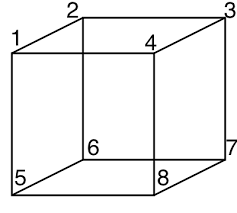
\includegraphics[width=3cm,height=3cm]{cube.png}
\centering
\caption{Cube with labeled vertices}
\end{figure}
\par
Consider a cube as shown in the figure. Here in one projection we will see that one one edge 1 may be mapped to 2 or 6 and it cannot be determined which of the two it has an edge with. To explain the problem more deeply, consider points 2 and 5. In the top view, due to the edge between 1 and 2, there is a line between 5 and 2 and it is not clear if an edge exists between the two. Similarly, in the front view, an edge between 1 and 5 leads to the same confusion. Thus it may not be possible to determine if an edge exists between the two. Only if we were given the side view would it be clear that an edge between the two exists or not. For simplification, in initial stages we may take edges defined in the projection to be defined as a tuple of vertices, doing away with this confusion.
\par In case, we are not given the edges as a tuple, it may be difficult to infer if an edge is present or not. We will first allow all such edges which cannot be determined to be present or not. Later such edges, which are not possible are removed. 
\subsection{3D view to Isometric}
In the isometric projection of a 3D object, all the three axes x-y-z are no longer orthogonal and there is a $120^{\circ}$ angle between each of the 3 axes. The isometric projection consists of two orthogonal U and V axes and each point in 3 dimensions can be mapped to this u-v plane. If we consider the axis U to be at angle $\alpha$ with the x-axis, the coordinates can be transformed using,
    \[\begin{bmatrix}u\\v\\\end{bmatrix} = \begin{bmatrix}\cos(\alpha) & cos(\alpha + 120^{\circ}) & cos(\alpha - 120^{\circ})\\sin(\alpha) & sin(\alpha + 120^{\circ}) & sin(\alpha - 120^{\circ})\\\end{bmatrix}\begin{bmatrix}x\\y\\z\\\end{bmatrix}\]
Here, $\alpha$ must be chosen appropriately, and we will chose it to be $30^{\circ}$ for simplicity.
\end{document}
